\section{Solutions}

\subsection{Solutions to T/F Questions}
	\begin{table}[!h]
		\centering
		\begin{tabular}{c@{\hspace{2.5em}}cp{0.75\textwidth}}
			true & false & \\
			\specialrule{\lightrulewidth}{0.25em}{1.25em}
			\bubble & \dbubble & If \(\lambda = 0\) is not an eigenvalue of a matrix, then the nullspace of that matrix is empty. \\[0.8em]
			\dbubble & \bubble & Every regular stochastic matrix has \(\lambda = 1\) as an eigenvalue.\\[0.8em]
			\dbubble & \bubble & If a matrix \(A\) can be row reduced to the identity matrix, it must be invertible.\\[0.8em]
			\dbubble & \bubble & If two square matrices \(A, B\) share an eigenvector \(\vec{v}\), where \(A\vec{v} = 2\vec{v}\) and \(B\vec{v} = \vec{v}\),
						      then \(\lambda = 5\) is an eigenvalue of the matrix \(2A + B\).\\[0.8em]
			\bubble & \dbubble & If \(B\) is an echelon form of a matrix \(A\), then the pivot columns of \(B\) form a basis for \(\colspace A\). \\[0.8em]
			\dbubble & \bubble & If \(A, B \in \mathbb{R}^{n\times n}\) with \(\det A = 1\) and \(\det B = -1\), then \(AB\) is invertible.\\[0.8em]
			\bubble & \dbubble & If \(A\) and \(B\) are invertible \(n \times n\) matrices, then \(AB = BA\). \\[0.8em]
			\bubble & \dbubble & If for all pair of vectors \(\vec{x}, \vec{y} \in \mathbb{R}^n\), \(A\vec{x} \ne A \vec{y}\), then 
						     \(\nullspace A \ne \{\vec{0}\}\). \\[0.8em]
			\bubble & \dbubble & The \(LU\) factorization for a given matrix is unique.\\[0.8em]
			\bubble & \dbubble & For any square matrix and any scalar \(c\), \(\det(cA) = c\det(A)\) \\[0.8em]
			\bottomrule
		\end{tabular}
	\end{table}

\subsection{Solutions to Possible/Impossible Questions}
	\begin{table}[!h]
		\centering
		\begin{tabular}{c@{\hspace{2.5em}}cp{0.75\textwidth}}
			possible & impossible & \\
			\specialrule{\lightrulewidth}{0.25em}{1.25em}
			\dbubble & \bubble & A non-invertible matrix A with a nonzero eigenvalue. \\[0.8em]
			\dbubble & \bubble & A matrix \(A\) that is both an upper triangular and lower trangular matrix. \\[0.8em]
			\dbubble & \bubble & \(A\) is a \(5 \times 3\) matrix with \(\rank A = 2 \cdot \dim(\nullspace(A))\).\\[0.8em]
			\bubble & \dbubble & Eigenvectors \(\vec{v}_1\) and \(\vec{v}_2\) of \(A\) that are scalar multiple of each other, but are from different
						      eigenspaces. \\[0.8em]
			\bubble & \dbubble & An \(n \times n\) matrix \(A\) that is both invertible and has \(\dim(\nullspace(A)) = 1\). \\[0.8em]
			\dbubble & \bubble & \(A\) is a non-zero matrix whose columns don't form a basis for \(\colspace A\). \\[0.8em]
			\dbubble & \bubble & \(A \in \mathbb{R}^{3 \times 3}\) and \(A\) has only 2 distinct eigenvalues.\\[0.8em]
			\bubble & \dbubble & \(A \in \mathbb{R}^{3 \times 2}\) and \(\colspace A = \mathbb{R}^3\).\\[0.8em]
			\bottomrule
		\end{tabular}
	\end{table}


\subsection{Solutions to Short/Long Answer Questions}
\begin{enumerate}
	\item[\textbf{Q1}] \[    \begin{pmatrix} A & 0 \\C & D\end{pmatrix} \begin{pmatrix}W & X \\Y & Z \end{pmatrix}
			= \begin{pmatrix} AW + 0Y & AX + 0Z \\ CW + DY & CX + DZ \end{pmatrix}
			= \begin{pmatrix} I & 0 \\ 0 & I \end{pmatrix}.\]
		\(AW = I \implies W = A^{-1}\). \(AX = 0  \implies X = 0\). \(CW + DY = 0 \implies DY = -CW \implies Y = -D^{-1}CA^{-1}.\) 
		\(CX + DZ \implies Z = D^{-1}\). Therefore, \[A^{-1} = \begin{pmatrix}A^{-1} & 0 \\ -D^{-1}CA^{-1} &  D^{-1}\end{pmatrix}.\]
	
	\item[\textbf{Q2}] When we row-reduce \(A\), we get \(U = \begin{pmatrix}1 & 2 & 2 \\ 0 & -4 & -6 \\ 0 & 0 & -1\end{pmatrix}\), and 
		\(L = \begin{pmatrix}1 & 0 & 0 \\ 4 & 1 & 0 \\ 4 & 1/2 & 1\end{pmatrix}\).
	
	\item[\textbf{Q3}] Row reduce \(\begin{bmatrix}A & | & I_3\end{bmatrix}\). 
		\[\left(\!\!\begin{array}{ccc|ccc}0 & 1 & 2 & 1 & 0 & 0 \\ 1 & 2 & 3 & 0 & 1 & 0 \\ 3 & 1 & 1 & 0 & 0 & 1\end{array}\!\!\right)
	\sim	  \left(\!\!\begin{array}{ccc|ccc}1 & 0 & 0 & 1/2 & -1/2 & 1/2 \\ 0 & 1 & 0 & -4 & 3 & -1 \\ 0 & 0 & 1 & 5/2 & -3/2 & 1/2\end{array}\!\!\right)
		\] So \(A^{-1} = \begin{pmatrix}1/2 & -1/2 & 1/2 \\ -4 & 3 & -1 \\ 5/2 & -3/2 & 1/2\end{pmatrix}\).
	
	\item[\textbf{Q4}] First solve for \(L\vec{y} = \vec{v}\), then for \(U\vec{x} = \vec{y}\). We get that \(\vec{x} = \begin{pmatrix}6\\-7\\2\end{pmatrix}\).

	\item[\textbf{Q5}] This is sneaky. Read to the end of this. 
		\[\begin{vmatrix}0 & x & 0 & y \\ -3 & 1 & 3 & 2 \\ 9p & 9q & 0 & 9 \\ 2 & 2 & 0 & 2\end{vmatrix} 
		= -3\begin{vmatrix}0 & x & y \\ 9p & 9q & 9 \\ 2 & 2 & 2\end{vmatrix}.\] Do you see why that is? (Perform cofactor expansion starting from the
		third column.) We see that the submatrix we've obtained and the given \(3 \times 3\) matrix are row equivalent. We scaled one of the rows by 2,
		performed one row swap operation, and then we scaled a row by 9. Therefore, the determinant is \(-3\cdot (6)(9)(-1)(2) = 324\).	
	\item[\textbf{Q6}] \(\det(A^2B^4)=16 \implies \det(A^2) \cdot \det(B^4)  = 16 \implies \det(A)^2 \cdot\det(B)^4 = 16 \implies \det(B) = \sqrt{2}.\) Now,
		what remains is to find \(\det C\). 
		\(C = 2AB \implies \det(C) = \det(2AB) \implies \det(C) = \det(2A) \cdot \det(B) \implies \det(C)=2^3\det(A)\cdot\det(B) \implies \det(C) = 16\sqrt{2}.\)
	\item[\textbf{Q7}] Yes.
		\begin{align*}
			\mathcal{C} = \left\{\!\left.\begin{pmatrix}a \\ a + b \\ b\end{pmatrix} \;\right|\; a, b \in \mathbb{R}\!\right\} &= \left\{\!\left.\begin{pmatrix}a \\ a \\ 0\end{pmatrix} + \begin{pmatrix}0 \\ b \\ b\end{pmatrix}\;\right|\; a, b \in \mathbb{R}\!\right\} \\ &= \left\{\!\left.a\begin{pmatrix}1 \\ 1 \\ 0\end{pmatrix} + b\begin{pmatrix}0 \\ 1 \\ 1\end{pmatrix}\;\right|\; a, b \in \mathbb{R}\!\right\}
		\end{align*}
		So, \(\mathcal{C} = \vspan \left\{\!\begin{pmatrix}1 \\ 1 \\ 0\end{pmatrix}, \begin{pmatrix}0 \\ 1 \\ 1\end{pmatrix}\!\right\}\). This is a 2-dimensional
		subspace.
	\item[\textbf{Q8}]
		\begin{align*}
			\mathcal{Q} = \{\vec{x} \in \mathbb{R}^3 \mid x_1 = -x_2\} &= \{\vec{x} \in \mathbb{R}^3 \mid x_1 + x_2 = 0\} \\
					 &= \{\vec{x} \in \mathbb{R}^3 \mid x_1 + x_2 + 0x_3 = 0\}.
		\end{align*}
		We see that \(\mathcal{Q} = \nullspace(\begin{bmatrix}1 & 1 & 0\end{bmatrix})\). We know that \(\dim(\nullspace \begin{bmatrix}1 & 1 & 0\end{bmatrix}) = 2 = \dim \mathcal{Q}.\)

	\item[\textbf{Q9}] Note: You can solve this problem \emph{just by looking at the matrix and the \(\vec{b}\) vector.} Do you see how? Otherwise, you can
			row reduce, and while your paramterization might be different, you should obtain the same lines.
		\begin{figure}[!h]
			\centering
			\begin{minipage}{0.33\textwidth}
				\centering
				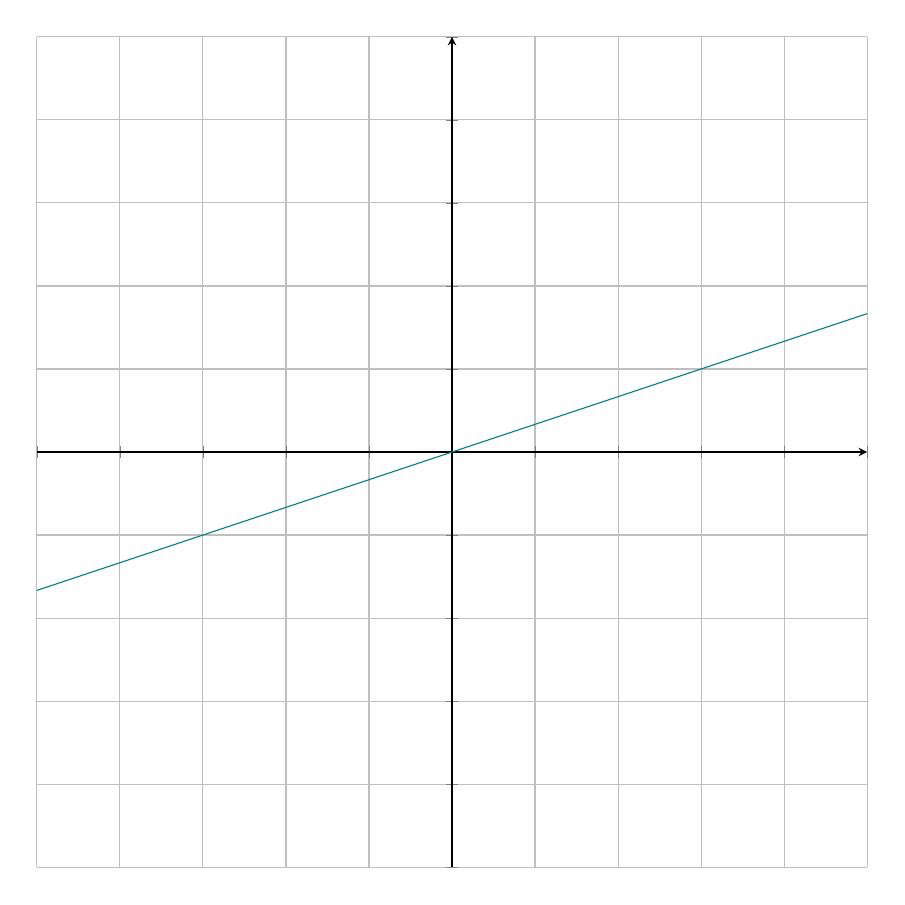
\begin{tikzpicture}
					\begin{axis}[axis lines = center, width=\textwidth, height=\textwidth, xmin=-5, xmax=5, ymin=-5, ymax=5, grid=major, xtick distance = 1, ytick distance = 1, xticklabel = \empty, yticklabel = \empty]
						\addplot[teal, domain=-5:5] {1/3*x};
					\end{axis}
				\end{tikzpicture}
				\caption{\(\nullspace A\).}
			\end{minipage}\hfill
			\begin{minipage}{0.33\textwidth}
				\centering

				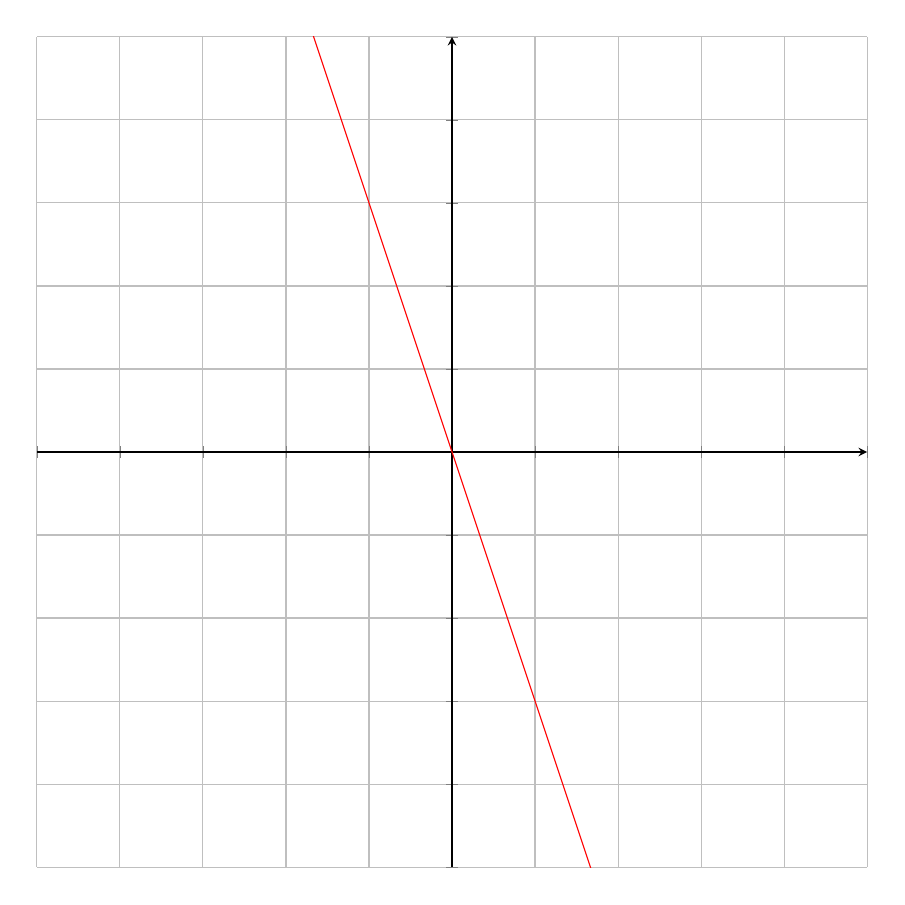
\begin{tikzpicture}
					\begin{axis}[axis lines = center, width=\textwidth, height=\textwidth, xmin=-5, xmax=5, ymin=-5, ymax=5, grid=major, xtick distance = 1, ytick distance = 1, xticklabel = \empty, yticklabel = \empty]
						\addplot[red, domain=-5:5] {-3*x};
					\end{axis}
				\end{tikzpicture}
				\caption{\(\colspace A\).}
			\end{minipage}\hfill
			\begin{minipage}{0.33\textwidth}
				\centering
				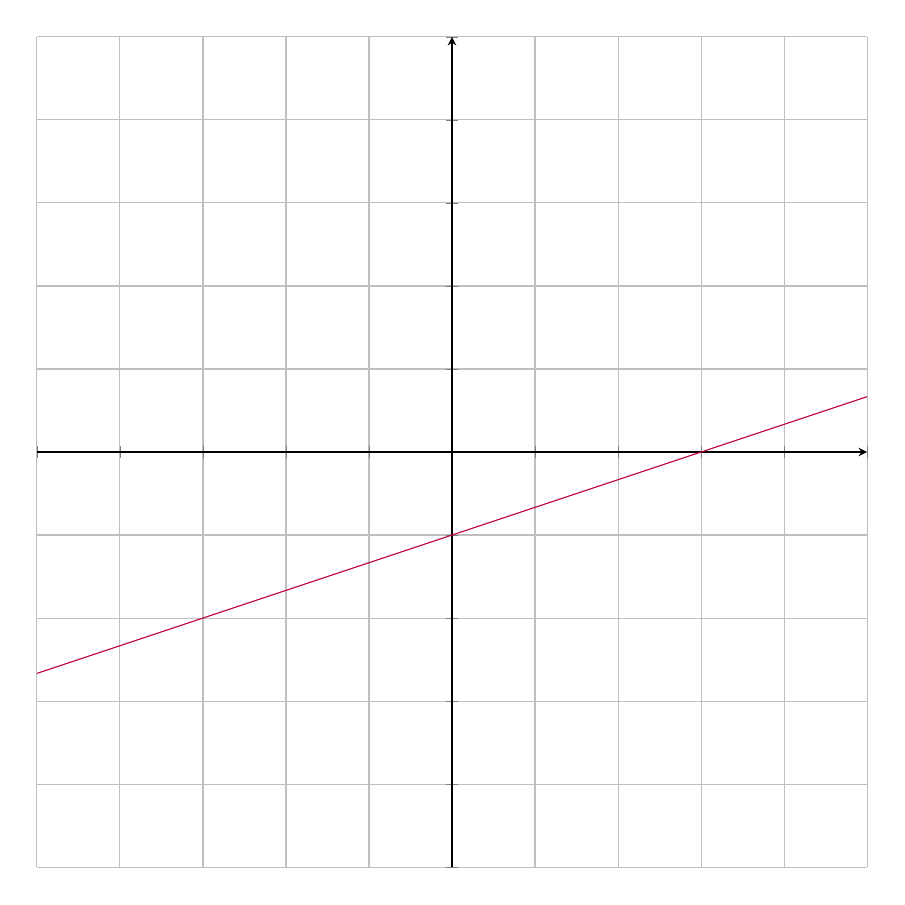
\begin{tikzpicture}
					\begin{axis}[axis lines = center, width=\textwidth, height=\textwidth, xmin=-5, xmax=5, ymin=-5, ymax=5, grid=major, xtick distance = 1, ytick distance = 1, xticklabel = \empty, yticklabel = \empty]
						\addplot[purple, domain=-5:5] ({3*x}, {x-1});
					\end{axis}
				\end{tikzpicture}
				\caption{Solutions to \(A\vec{x} = \vec{b}\).}
			\end{minipage}
		\end{figure}

	\item[\textbf{Q10}] \(A\vec{u} \ne \vec{0}\), so \(\vec{u} \notin \nullspace A\). To check (b), note that we're wondering if there exists at least one set of 
		scalars \(c_1, c_2, c_3\) such that \[c_1\begin{pmatrix}1 \\ -4 \\ -3\end{pmatrix} + c_2\begin{pmatrix}-3 \\ 6 \\ 7\end{pmatrix} + c_3\begin{pmatrix}-4 \\ 2 \\ 6\end{pmatrix} = \begin{pmatrix}3 \\ 3 \\ -4\end{pmatrix} = \vec{u}.\] Which is the same as wondering if \(A\vec{c} = \vec{u}\) is
		consistent. So, we row reduce the matrix \(\begin{bmatrix}A & | & \vec{u}\end{bmatrix}\). Since this system is consistent, we find that there
		\emph{does} exist a set of scalars that satisfy the vector equation, so the answer to (b) is yes. To answer (c), row reduce \(A\). The pivotal columns
		of \(A\) then form a basis for \(\colspace A\). In this case, the set below forms a basis for \(\colspace A\). Every column of \(A\) is pivotal, so the 
		columns of\(A\) form a basis for \(\colspace A\).

	\item[\textbf{Q11}] Let's ignore the prompt and try to find the eigenvalues of the matrix \(A\). 
		\[A - \lambda I = \begin{pmatrix}-\lambda & k \\ 2  & 4 - \lambda\end{pmatrix}, 
		\qquad \begin{vmatrix}-\lambda & k \\ 2  & 4 - \lambda\end{vmatrix} = \lambda(4+\lambda) - 2k.\]
		The characteristic equation is therefore \(\lambda^2 + 4\lambda - 2k = 0\). If our eigenvalue has an algebraic multiplicity of 2, it must satisfy the
		equation in the form of \((\lambda + a)^2\). In other words, we should be able to factor this quadratic polynomial as the square of a monomial.
		The only value that does this is \(k = -2\), because then, \(\lambda^2 + 4\lambda + 4 = (\lambda + 2)^2\). So we'd have an eigenvalue 
		\(\lambda = -2\) with an algebraic multiplicity of 2.

	\item[\textbf{Q12}]  There are actually multiple valid answers for this question. So, please note the states the columns correspond to.
			\NiceMatrixOptions{
				code-for-first-row=\color{teal},
				code-for-first-col=\color{purple},
			}
			\[
				\begin{bNiceMatrix}[first-row,first-col]
				   	&   A   &   B   &    C   \\
				     A & 0.5  & 0.25 & 0.2 \\
				     B & 0.5  &  0.5  & 0.5 \\
				     C &  0   &  0.25 & 0.3
				\end{bNiceMatrix}
			\]
			The states in teal denote the {\color{teal} from}, and the states in purple denote the states that {\color{purple} receive}.
		\item Finding the ``long-term trend" of the chain corresponds to finding the steady-state vector. 
			\begin{align*}
				\begin{bmatrix}0.5 & 0.25 & 0.2 \\ 0.5 & 0.5 & 0.5 \\ 0 & 0.25 & 0.3\end{bmatrix} - I_3 &= 
				\begin{bmatrix}-0.5 & 0.25 & 0.2 \\ 0.5 & -0.5 & 0.5 \\ 0 & 0.25 & -0.7\end{bmatrix} 
				\sim \begin{bmatrix}0.5 & -0.5 & 0.5 \\ 0 & -0.25 & 0.7 \\ 0 & 0.25 & -0.7\end{bmatrix} \\[0.5em]
				&\sim \begin{bmatrix}1 & -1 & 1 \\ 0 & 1 & - 14/5 \\ 0 & 0 & 0\end{bmatrix} 
				\sim \begin{bmatrix}1 & 0 & 1 - 14/5 \\ 0 & 1 & -14/5 \\ 0 & 0 & 0\end{bmatrix}
			\end{align*}
			From here we see that \(\vec{x} = t\begin{bmatrix}9/5 \\ 14/5 \\ 1\end{bmatrix}.\) However, the sum of the entries should add up to one, and
			so \(\vec{q} = \displaystyle \frac{5}{28}\begin{bmatrix}9/5 \\ 14/5 \\ 1\end{bmatrix}.\)
		
			You can verify that this is the steady-state vector by left-nultiplying it with the matrix. Note that \(\det(P - I) = 0\). (Why?)

\end{enumerate}